\documentclass{article}
\usepackage[utf8]{inputenc}

\title{udacity-nanodegree-estimation}
\author{Sumedh V Joshi }
\date{August 2020}

\usepackage{natbib}
\usepackage{graphicx}

\begin{document}

\maketitle

\section{Introduction}
This report discusses the various methods implemented in the udacity drone estimator project. In the controller project, it was assumed that all the sensors are perfect (without any noise or measurement error) and hence the estimated positions, velocities were always exact. This is very rarely the case with real sensors. Hence, in the following project, the following workflow has been adapted;

\begin{enumerate}
    \item Initially, the measurements of the GPS and accelerometer in X direction are analyzed to fully understand the concept of noise in a sensor. 
    \item The EKF process begins from here. Initially, a better attitude estimator is implemented which accounts for non-linearity's in measurements. 
    \item Next, the predict step for the estimator is implemented. This starts with defining the new covariance value for the state of the drone. The state mean and covariance from the previous time step and the current thrust vector. 
    \item Then the individual sensor measurements are read (GPS, magnetometer and so on).
    \item Finally, these new sensor measurments, state covariance and mean values from predict step are used to update the final state mean and covariance values.
\end{enumerate}

\section{Analysing sensor data for X position and velocity}
After running scenario 6 in C++, the generated txt. data is imported into an excel file. The Standard deviation function in excel was directly used to calculate the respective values.

\section{Predict state}
For the predict state, the classical EKF equation mentioned in the reference pdf, estimation for quadrotors has been implemented. 

\section{GPS and magnetometer update}
The update function is also implemented in exactly the similar way as described in the estimation for quadrotors pdf. 

\section{Estimator and controller}

In this section, I have used the controller implemented in the previous project in conjunction with the estimator. The sensors are modelled with noise, hence it is difficult to exactly estimate the position of the drone. This in turn leads to small changes in the thrust values obtained from the controller. Hence, the drone does not follow an exact square path and instead treads along a slightly different path but within the allowed deviation range. The results from scenario 11 are shown below.

\begin{figure}[h!]
\centering
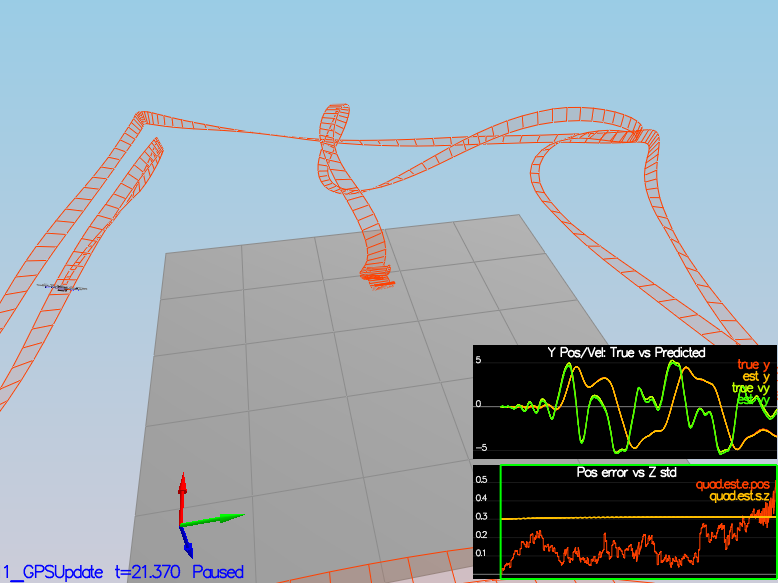
\includegraphics[scale=0.4]{scenario_11_1.PNG}
\caption{Scenario 11}
\label{fig:Scenario 11}
\end{figure}

\begin{figure}[h!]
\centering
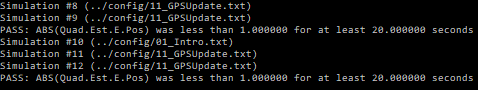
\includegraphics[scale=0.6]{scenario_11_2.PNG}
\caption{Scenario 11-B}
\label{fig:Scenario 11-B}
\end{figure}

\bibliographystyle{plain}

\end{document}
